\documentclass{elektr}
\usepackage{hyperref}
\hypersetup{
colorlinks=true,
urlcolor=blue,
citecolor=blue}
\usepackage[all]{xy,xypic}
\usepackage{amsfonts,amssymb,amsmath,amsgen,amsopn,amsbsy,theorem,graphicx,epsfig}
\usepackage{eufrak,amscd,bezier,latexsym,mathrsfs,eurosym,enumerate}
\usepackage[utf8]{inputenc}
\usepackage[english]{babel}
\usepackage{cleveref,multirow}
\usepackage[pagewise]{lineno}
\linenumbers


\usepackage{subfig}
\usepackage{wrapfig}
\usepackage{txfonts}
\usepackage{wasysym}
\usepackage{enumitem}
\usepackage{adjustbox}
\usepackage{ragged2e}
\usepackage[svgnames,table]{xcolor}
\usepackage{tikz}
\usepackage{longtable}
\usepackage{changepage}
\usepackage{setspace}
\usepackage{hhline}
\usepackage{multicol}
\usepackage{tabto}
\usepackage{float}
\usepackage{multirow}
\usepackage{makecell}
\usepackage{fancyhdr}
\usepackage[toc,page]{appendix}
\usetikzlibrary{shapes.symbols,shapes.geometric,shadows,arrows.meta}
\tikzset{>={Latex[width=1.5mm,length=2mm]}}
\usepackage{flowchart}\usepackage[paperheight=11.69in,paperwidth=8.27in,left=0.98in,right=0.98in,top=0.98in,bottom=1.47in,headheight=1in]{geometry}
\usepackage[utf8]{inputenc}
\usepackage[T1]{fontenc}
\TabPositions{0.49in,0.98in,1.47in,1.96in,2.45in,2.94in,3.43in,3.92in,4.41in,4.9in,5.39in,5.88in,}

\yil{}
\vol{}
\fpage{}
\lpage{}
\doi{}

\title{Automatic Localization of Cephalometric Points using Convolutional Neural Networks}

\author[M N Mohamed NOURDINE and Betül UZBAŞ]{
\textbf{M N Mohamed NOURDINE$^{1}$\thanks{mohamednjikam25@yahoo.com}~, Betül UZBAŞ$^{1,2}$}\\
$^{1}$Department of Computer Engineering, Faculty of Engineering and Natural Science, Konya Technical University, Konya, Turkey, \\ ORCID iD: https://orcid.org/0000-0001-7068-9323\\
$^{2}$Department of Computer Engineering, Faculty of Engineering and Natural Science, Konya Technical University,\\ Konya, Turkey, ORCID iD: https://orcid.org/0000-0002-0255-5988
\\ [1.8em]

\rec{.201}
\acc{.201}
\finv{..201}
}

\def\E{\ifmmode{\mathbb E}\else{$\mathbb E$}\fi} %natural numbers
\def\N{\ifmmode{\mathbb N}\else{$\mathbb N$}\fi} %natural numbers
\def\R{\ifmmode{\mathbb R}\else{$\mathbb R$}\fi} %real numbers
\def\Q{\ifmmode{\mathbb Q}\else{$\mathbb Q$}\fi} %rational numbers
\def\C{\ifmmode{\mathbb C}\else{$\mathbb C$}\fi} %complex numbers
\def\H{\ifmmode{\mathbb H}\else{$\mathbb H$}\fi} %complex numbers
\def\Z{\ifmmode{\mathbb Z}\else{$\mathbb Z$}\fi} %integers
\def\P{\ifmmode{\mathbb P}\else{$\mathbb P$}\fi} %real numbers
\def\T{\ifmmode{\mathbb T}\else{$\mathbb T$}\fi} %real numbers
\def\SS{\ifmmode{\mathbb S}\else{$\mathbb S$}\fi} %real numbers
\def\DD{\ifmmode{\mathbb D}\else{$\mathbb D$}\fi} %real numbers

\renewcommand{\a}{\alpha}
\renewcommand{\b}{\beta}
\renewcommand{\d}{\delta}
\newcommand{\D}{\Delta}
\newcommand{\e}{\epsilon}
\newcommand{\var}{\varepsilon}
\newcommand{\g}{\gamma}
\newcommand{\la}{\lambda}
\newcommand{\La}{\Lambda}
\newcommand{\lan}{\langle}
\newcommand{\ran}{\rangle}
\newcommand{\n}{\nabla}
\newcommand{\va}{\varphi}
\newcommand{\s}{\sigma}
\newcommand{\Sig}{\Sigma}
\renewcommand{\t}{\tau}
\renewcommand{\th}{\theta}
\newcommand{\Om}{\Omega}
\newcommand{\om}{\omega}
\newcommand{\pa}{\partial}
\newcommand{\up}{\upsilon}
\newcommand{\vp}{\varphi}
\newcommand{\z}{\zeta}





\newcommand{\bse}{\begin{subequations}}
\newcommand{\ese}{\end{subequations}}
\newcommand{\ben}{\begin{enumerate}}
\newcommand{\een}{\end{enumerate}}
\newcommand{\bens}{\begin{enumerate*}}
\newcommand{\eens}{\end{enumerate*}}
\newcommand{\be}{\begin{equation}}
\newcommand{\ee}{\end{equation}}
\newcommand{\bea}{\begin{eqnarray}}
\newcommand{\eea}{\end{eqnarray}}
\newcommand{\baa}{\begin{eqnarray*}}
\newcommand{\eaa}{\end{eqnarray*}}
\newcommand{\bc}{\begin{center}}
\newcommand{\ec}{\end{center}}
\newcommand{\ol}{\overline}
\newcommand{\ul}{\underline}
\newcommand{\ov}{\overbrace}
\newcommand{\uv}{\underbrace}
\newcommand{\Ra}{\Rightarrow}
\newcommand{\ra}{\rightarrow}
\newcommand{\ds}{\displaystyle}
\newcommand{\vs}{\vspace}


\newcommand{\IR}{\mbox{I \hspace{-0.2cm}R}}
\newcommand{\IN}{\mbox{I \hspace{-0.2cm}N}}



%% \theoremstyle{plain} %% This is the default

\newtheorem{theorem}{Theorem}%[section]

\theoremstyle{corollary}
\newtheorem{corollary}{Corollary}

\theoremstyle{lemma}
\newtheorem{lemma}{Lemma}

\theoremstyle{proposition}
\newtheorem{proposition}{Proposition}

\theoremstyle{axiom}
\newtheorem{axiom}{Axiom}

\theoremstyle{conjecture}
\newtheorem{conjecture}{Conjecture}

\theoremstyle{example}
\newtheorem{example}{Example}

\theoremstyle{definition}
\newtheorem{definition}{Definition}%[section]

\theoremstyle{remark}
\newtheorem{remark}{Remark}%[section]
\newtheorem{notation}{Notation}


\newtheorem{question}{Question}%[section]
\newtheorem{construction}{Construction}

\newtheorem{athm}{Theorem}
\renewcommand{\theathm}{\Alph{athm}}





\setcounter{page}{1}
\begin{document}

\maketitle


\begin{abstract}Today, a large amount of data is collected using computers in every sector especially in areas such as health, defense industry, space and cybersecurity. With the increase in research in digital x-ray imaging, experts have successfully brought forward interesting and effective methods to address critical medical analysis problems. One of this field is cephalometric analysis. Cephalometric analysis is the process of determining a set of landmarks on lateral cephalograms. This process plays an important role in clinical analysis of tooth and skeletal relationships of the human skull and facilitates the interpretation of the bone, tooth and soft tissue structures of the patient. It is widely used during the process of dental treatment diagnosis, planning and surgery. It is also used during oral, craniofacial and maxillofacial surgery and during orthodontic treatments in orthodontic and orthopedic departments. The automatic localization of these points reduces possible human errors and is greatly time saving giving room for a more accurate analysis. To address this issue in a more convenient way, a deep learning model has been propose inspired from U-Net model. 400 cephalometric X-ray images dataset created under the context of the IEEE 2015 International Symposium on Biomedical Imaging (International Symposium on Biomedical Imaging, ISBI 2015) is used for this experience. The 19 cephalometric points on images which are generally manually determined by experts are automatically obtained using this model. This work was made possible using the personalized U-Net model and the results of the proposed model were compared with those found by experts in this competition context. A Success Detection Rate (SDR) of 74$\%$  in the range of 2 mm was achieved, 81.4$\%$  in the 2.5mm range, 86.3$\%$  in the 3mm range and 92.2$\%$  SDR in the 4mm range.
	

\keywords{Convolutional Neural Networks, Cephalometric Points Detection, Cephalometric landmarks, Medical Image Analysis, Success Detection Rate (SDR)}
\end{abstract}

\section{Introduction}
\label{Int} \tab Cephalometric analysis is a basic tool of clinical assessment in modern craniofacial, oral and maxillofacial surgery and during orthodontic treatment. It is the scientific measurement of the dimensions of an x-ray lateral cephalogram which are the main resources in this analysis\cite{ref1}. Cephalometric analysis is widely used in orthodontics and orthopedic sections as it measures the tooth and skeletal relationships of the human skull and facilitates the orthodontic analysis, treatment planning and interpretation of bone, tooth and soft tissue structures of the patients. It is initially done though the mathematical assessment of the regions among the teeth, jaws, maxilla and the mandible, using this information to give the accurate position of the landmark points. The positions of these points generally plays a very vital role during treatment planning, assessment of curative effect and to compare different cases.

In general, cephalometry points localization are manually computed by physicians, medical doctors or clinicians. This procedure is studios and time consuming as it takes a relatively long time for a very experienced doctor to accurately go through a lateral cephalogram and deduce these points in a consistent and accurate way. In addition, the points detected by different experts can often be inconsistent. Since there is no special interpolation formular for this operation and the images differing from one to another, the results obtained after hours of calculations may suffer from intra-observer variability since different doctors may differ considerably in their identification of landmarks \cite{ref2}. To solve this problem and to provide more reliable results, attempts have been made by researchers to automatically detect cephalometric points in order to overcome these limitations in clinical practice and research environment. This operation is a difficult task mainly due to the structure of the data. 

\section{Related Work}

\tab In general, cephalometry points localization are manually computed by physicians, medical doctors or clinicians. This procedure is studios and time consuming as it takes a relatively long time for a very experienced doctor to accurately go through a lateral cephalogram and deduce these points in a consistent and accurate way. In addition, the points detected by different experts can often be inconsistent. Since there is no special interpolation formular for this operation and the images differing from one to another, the results obtained after hours of calculations may suffer from intra-observer variability since different doctors may differ considerably in their identification of landmarks \cite{ref2}. To solve this problem and to provide more reliable results, attempts have been made by researchers to automatically detect cephalometric points in order to overcome these limitations in clinical practice and research environment. This operation is a difficult task mainly due to the structure of the data. 

As earlier mentioned, significant progress has been made towards automatically detecting points and pattern structures in radiographic x-ray images. These approaches are done by either specifying rules based on known rules or experts’ knowledge or using templates gray-scales morphological operators to regress the cephalometric points. In order to boost the research in this field, in 2014 and 2015 the International Symposium on Biomedical Imaging (ISBI) launched challenges on cephalometric landmark detection and several researches took part and propose different technics to achieve this operation. 

One of the most prominent results validated during this competition was the one developed by \cite{ref3}. It was based on random-forest and it achieved a success detection rate of 73.7$\%$  for a 2 mm precision range. Another prominent study retained during this competition was that of \cite{ref4} which obtained the second highest result with a success detection accuracy of 71.7$\%$  withing a 2 mm range. The method they used was to apply a Haar-like feature extraction with a random forest regression and continued making adjustments with a global context shape model.

Later on, in the process of landmarks localization, many other researchers tried some other technics. One of these is the work proposed by \cite{ref5} who developed a grayscale morphology and template matching algorithm. Using Dynamic programming, they exploited and applied the templates to the extract the cranial contour on high resolution X-Ray cephalometric images. In total, 20 landmarks were detected using this approach. They concluded by testing their work on 40 x-rays images which showed 85$\%$  recognition rate on average. 

Another prominent model architecture called CephaNet was proposed in 2019 by \cite{ref1}. In CephaNet, they designed a multi-task loss for reducing intra-class variations which adopted the multi-scale training strategy with the aim of improving the detection accuracy of small landmarks range. With this method, the obtained a success detection accuracy of 82.5$\%$  within the 2 mm range.

In the same line of work,\cite{ref6} proposed a different approach that successfully regressed the x and y coordinates of the landmarks directly from the cephalometric image. For each normalized coordinate variable, a CNN-based regression system was trained and corresponding coordinate variable, which is a variable to be regressed. They trained 38 regression systems with the same CNN structure on coordinate variables, respectively. Finally, they computed 38 coordinate variables with these trained systems from unseen images and extract 19 landmarks by pairing the regressed coordinates.\ They obtained a success detection rate (SDR) of 86.4 $\%$  on 2mm.   

\section{Architecture of the Proposed Model}

\tab In this study, we equally propose a CNN base approach that regress the coordinates of cephalometric based on a specialized U-Net model and then we compare the results obtained with the results accepted during the International Symposium on Biomedical Imaging (ISBI) competition. The Success Detection Rate of our system is evaluated using the evaluation metrics used during the competition. These includes 2 mm, 2.5 mm, 3 mm and 4 mm range around the landmark point. 

\subsection{Material and Method}

\tab In medical imaging tasks, CNN have proven to be really good when it comes to tasks like segmentation of organs, lesions and tumors \cite{ref7}. It is also a promising field for image classification tasks, image enhancement and construction. In the approach proposed, the coordinates of cephalometric points are determined using a multilayered model inspired by U-Net. 


\subsubsection{Cephalometric Signal Localization}
\tab Cephalometric analysis is the process that allows clinicians to interpret patients’ bone, tooth and soft tissue structures in a cephalometric or dental X-ray images. Figure (\ref{fig1}) below is a cephalometric image and shows cephalometric points marked on it which will be obtained automatically using specialized U-Net model within the scope of this research.


%%%%%%%%%%%%%%%%%%%% Figure/Image No: 1 starts here %%%%%%%%%%%%%%%%%%%%

\begin{figure}[H]
	\begin{center}
		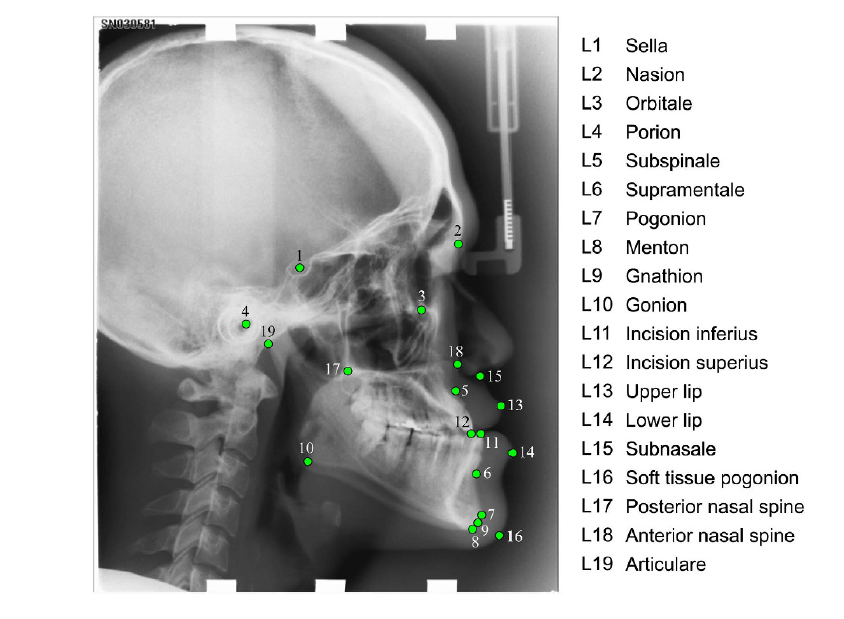
\includegraphics[width=5.76in]{./media/image1}
		\caption{Cephalogram annotation example showing the 19 landmark position used in this study.  (Lindner et al., 2016)}
		\label{fig1}
	\end{center}\vs{-4mm}
\end{figure}


%%%%%%%%%%%%%%%%%%%% Figure/Image No: 1 Ends here %%%%%%%%%%%%%%%%%%%%



\subsubsection{Dataset}
\tab The data used in the scope of this research are obtained from publicly available dataset provided during the 2015 ISBI Grand Challenge Training Dataset. It contained 400 Lateral Cephalometric images with patients mean age being 27 years with an age range of 7 to 76. These data were collected from 235 females and 165 males. All cephalograms were acquired in TIFF format with a Soredex CRANEXr Excel Ceph machine (Tuusula, Finland) using Soredex SorCom software (3.1.5, version 2.0) (Lindner et al., 2016). The image resolution is 1935 $ \times $  2400 pixels with a pixel spacing of 0.1 mm. The images are primarily labeled by a senior and a junior doctor and the annotation results made available in two different folders. We used the annotations from the senior doctor for more convenience and aim to detect 19 landmarks for each X-ray image, as presented in Figure (\ref{fig1}), which are as follows: sella turcica, nasion, orbitale, porion, subspinale, supramentale, pogonion, menton, gnathion, gonion, lower incisal incision, upper incisal incision, upper lip, lower lip, subnasale, soft tissue pogonion, posterior nasal spine, anterior nasal spine, and articulate. The authors of this symposium have divided the dataset into three groups of images: the training set contains 150 images, the test1 which contains 150 images and the test2 which contains 100 images. 

The images used during this experiment were resized to 256x256 px sizes that is one-eight of the original size. 

\subsubsection{Data Augmentation}
\label{DataAugmentation}
\tab In order to increase the accuracy of our model, data augmentation was performed on the training dataset which initially comprised of 150 annotated images. This operation conveniently boosted the model by permitting it to learn more efficiently. The data augmentation is performed on the dataset was a shifting\  1 and 3 pixels in 4 different directions (right, left, down, up) on 256x256 pixels cephalometric image. Every image on the training dataset is shifted using this shift metrics and one images generates 4 new images with the new coordinates. This operation is performed using the famous library for image augmentation called Imgaug (Jung, 2018). After performing the data augmentation on the images, we successfully generated a total of 1350 images used for training. 

\subsection{U-Net Network Architecture}
\tab U-Net (Ronneberger, Fischer, $\&$  Brox, 2015) is the CNN architecture presented in 2015 to address the issue of biomedical image processing, classification and segmentation. The U-net model initially used for segmentation of neural structures was considered as one of the best methods in ISBI cell tracking challenge in 2015 (Goutham, Vasamsetti, Kishore, $\&$  Sardana, 2019). 


\begin{adjustwidth}{0.40in}{0.24in}
	\subsubsection*{The proposed model }
	\addcontentsline{toc}{subsubsection}{The proposed model }
\end{adjustwidth}


The CNN architecture proposed for the purpose of this study follows closely the U-Net model with slight modification to achieve more efficiency. It is experiment on the augmented training dataset and evaluated using test1 dataset. This test dataset was not used to give room to a reliable result comparison with results accepted for the ISBI Challenges. It is made up of a down sampling layers which are followed by a symmetric up sampling layer path. It is designed to learn the local characteristics of each landmark gradually in both directions. It has as input dimension of 256x256x1. Figure (\ref{fig2}) shows the customized U-Net architecture development for this task.



%%%%%%%%%%%%%%%%%%%% Figure/Image No: 2 starts here %%%%%%%%%%%%%%%%%%%%
\begin{figure}[H]
	\begin{center}
		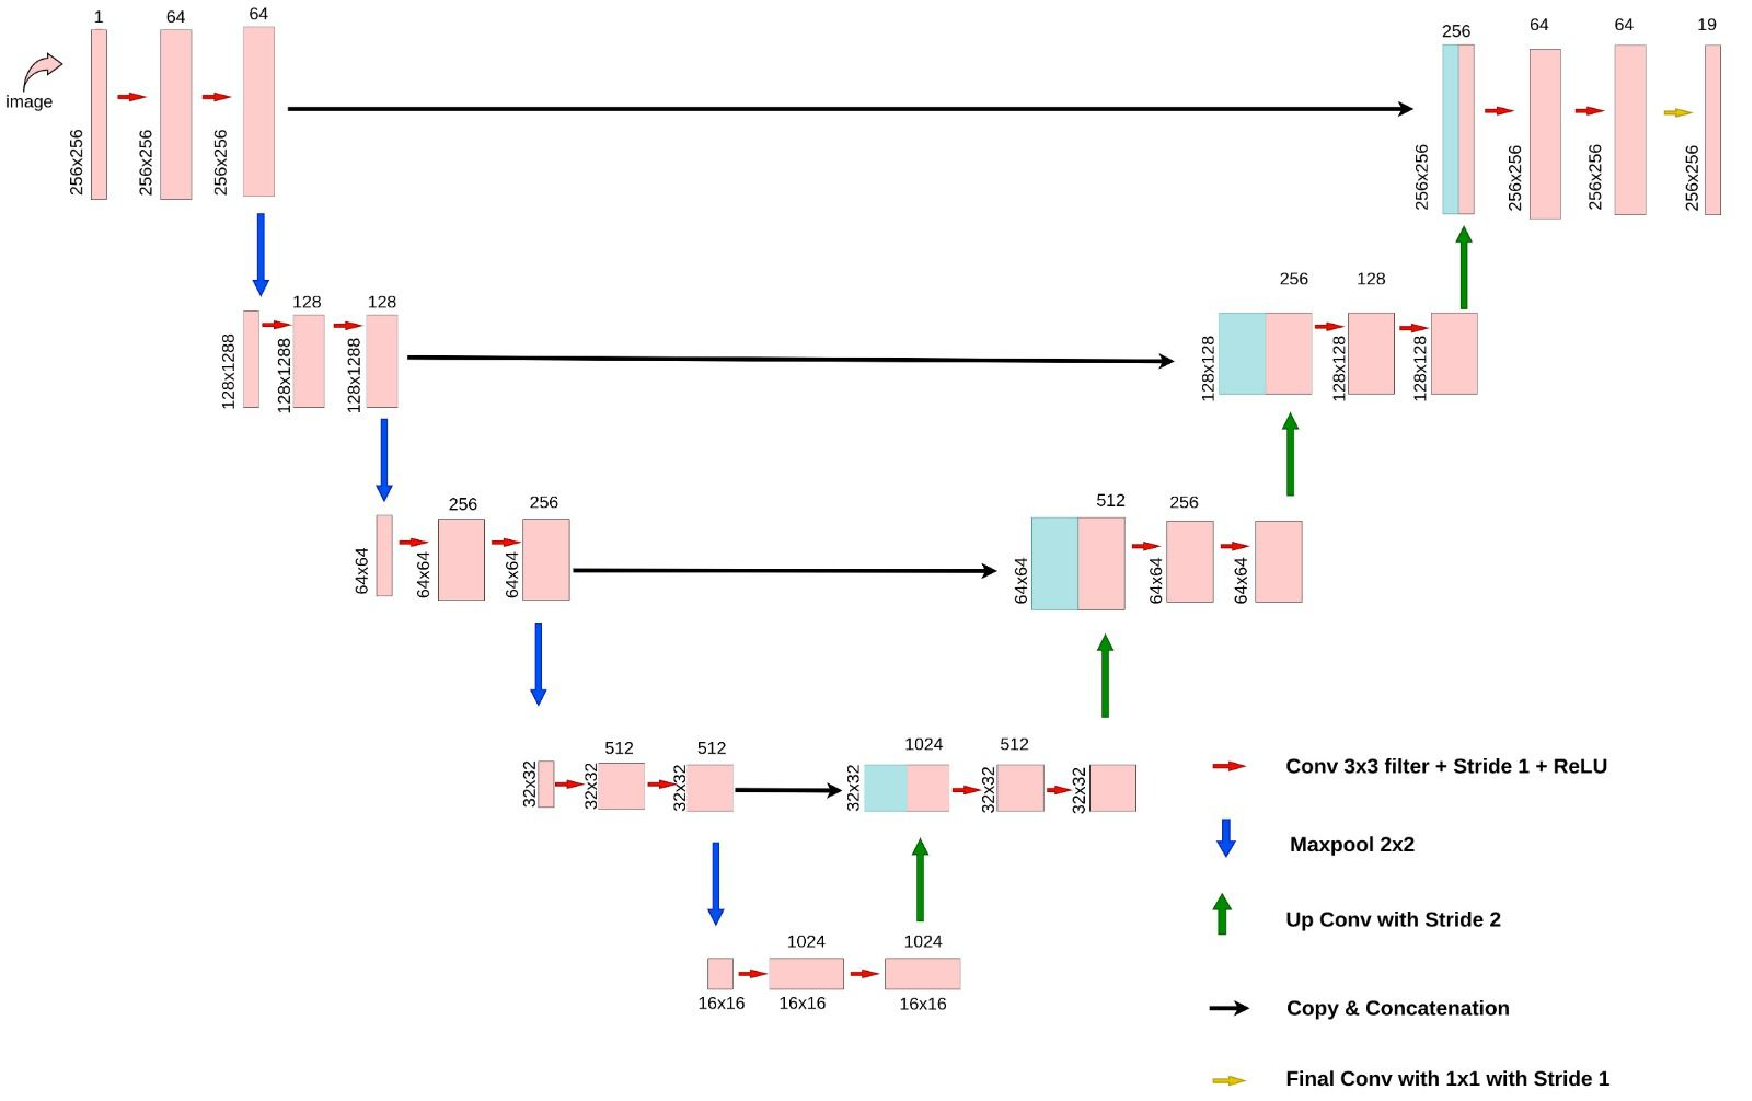
\includegraphics[width=6.3in]{./media/image2}
		\caption{Architecture of the Proposed Model}
		\label{fig2}
	\end{center}\vs{-4mm}
\end{figure}



%%%%%%%%%%%%%%%%%%%% Figure/Image No: 2 Ends here %%%%%%%%%%%%%%%%%%%%

As shown in figure (\ref{fig2}) above, the propose model is divided into three main blocks; the down sampling block, bottleneck and the up-sampling block.

Applying down sampling to the dimensions of input images reduces resolution and allows the network to learn more properties on the image, which includes information about the relative positions of the place marks. It consists of subsequent 2 convolution layers with kernel size of 3x3 follows by a stride of 1 and padding of 1 and a non-linear activation function layer using the rectifier linear unit ReLU. It is then followed by an average pooling layer. The block size is of height 4 till the bottleneck. In this phase, the channel size of the input image is first expanded using a pair of Convolutional that allow the network to model richer properties in this down sampling phase. The maximum pooling layer halves the width and height dimensions of the property map. Each down sampling level follows a similar pattern where the input property is passed through a double convolution which is responsible to increase the number of its channels by two before it is passed through a max pooling layer. The filter sizes used for this operation 4 till the bottleneck are 64,128,256,512,1024. The bottleneck layer is the base turn point for the model and consists of 1024 filters. The up-sampling path consists of the applying a transpose convolution to the lower feature map which then doubles its dimensions thus the channel size. This model repeats for each level in the up-sampling path. In the final layer at the highest level, it uses 1$ \times $ 1 filter to create the landmark heatmaps space as model predictions. It is worth mentioning that a batch normalization layer is applied after every convolutional layer’s ReLU activation to speed up the training process. 

Input to CNN is a single-channel gray scale image. All models are trained as 256x256 image size to provide faster training times and easier evaluation. The application was developed using the PyTorch (Paszke et al., 2017) framework on a 64-bit Intel® Core™ i7-9700F CPU @ 3.00GHz 3.00GHz 16.0GB RAM Computer. 


%%%%%%%%%%%%%%%%%%%% Figure/Image No: 3 starts here %%%%%%%%%%%%%%%%%%%%

\begin{figure}[H]
	\begin{center}
		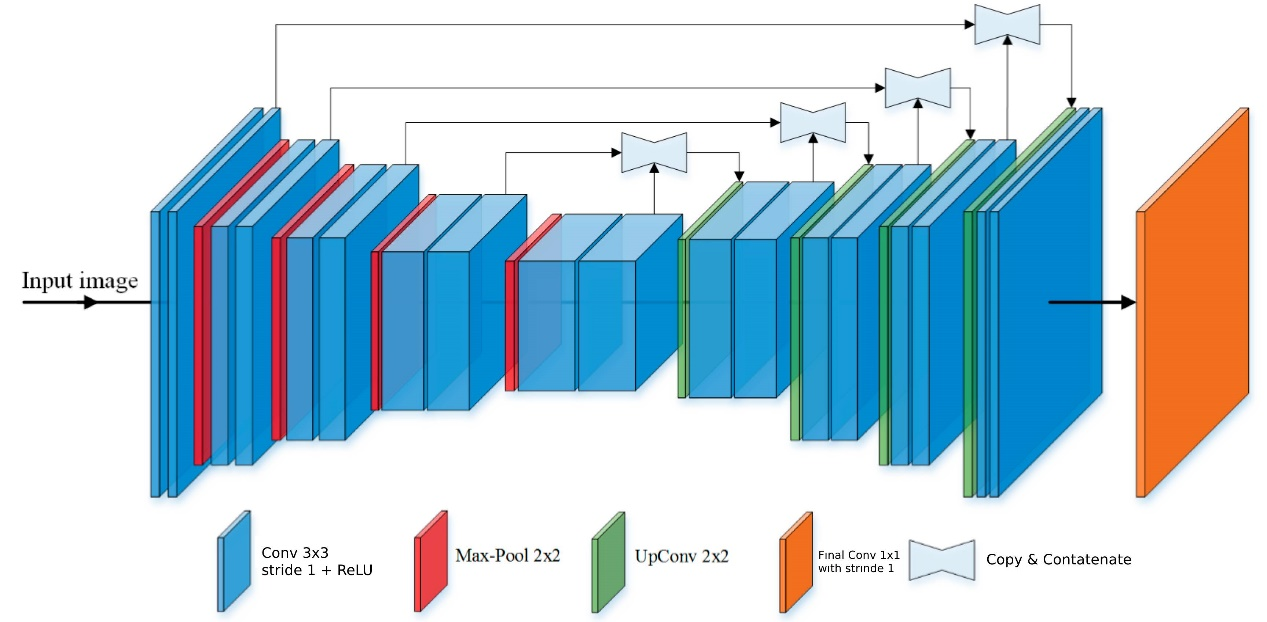
\includegraphics[width=5.76in]{./media/image3}
		\caption{Block Architecture of the Proposed Model. (Original Image from (Ye et al., 2019))}
		\label{fig2}
	\end{center}\vs{-4mm}
\end{figure}

%%%%%%%%%%%%%%%%%%%% Figure/Image No: 3 Ends here %%%%%%%%%%%%%%%%%%%%


Adam Optimization (Kingma $\&$  Ba, 2014) was used for optimizing training with a batch size of 8. The initial learning rate of the model was set to  \( 10^{-3} \)  and the weight decay of  \( 10^{-4} \)  to overcome the problem of overfitting during training. The model was trained on 85$\%$  of the training data and validated on 15$\%$ . If the performance in terms of validation loss did not improve for 10 consecutive epochs the learning rate was decrease by 10 and the training process was restarted. This action was done and stop after 10 consecutive epochs where the validation loss did not change.

\subsection{Evaluation Metrics}

\tab Landmark localization model performance is evaluated using the same measurements used for the ISBI 2015 competition. Using these metrics, the models we train are comparable to those who retained in the ISBI competition.

\tab The loss of MSE \textbf{(Mean Square Error)} has been used to train models for the heatmap regression:



\begin{equation}
	\label{eq1}
	MSE=\frac{1}{m} \sum _{i=1}^{m} \left( y-\hat{y} \right) ^{2}
\end{equation}

In equation (\ref{eq1}) above, \( y \) are the ground truth heatmaps and  \( \hat{y} \)  are the model predictions,  \( m \)  is the batch size. The ground truth heatmap values come from the annotations of the physicians. The neural network focuses on predicting a zero-filled heatmap and ignores the one set to 1. In order to fasten the training operation and facilitates the model’s convergence, the Gaussian at the landmark position and the loss function’s gradient in the area around the landmark position was increased. For training images of size 256$ \times $ 256, the best-performing Gaussian had an amplitude of 1000 and standard deviation of 5. 


The \textbf{Mean Radial Error (MRE)} and the \textbf{Standard Deviation (STD)} values are evaluated for performance measures. The Radial Error R is the Euclidean Distance between the predicted position  \( y \)  and actual landmark position  \( x \) 


\begin{equation}
	\label{eq2}
	R=\sqrt[]{ \Delta x^{2}- \Delta }\overline{y^{2}}
\end{equation}

\tab In equation (\ref{eq2}) above, \(  \Delta x \)  and  \(  \Delta y \) , are the distances between the actual bookmark position and the predicted position. 


\tab Associated with Mean Radial Error (MRE) and Standard Deviation (STD)

\begin{equation}
	\label{eq3}
	MRE=\frac{ \sum _{i=1}^{N}R_{i}}{N}
\end{equation}

\begin{equation}
	\label{eq4}
	STD=\sqrt[]{\frac{ \sum _{i=1}^{N} \left( R_{i}-MRE \right) ^{2}}{N}}
\end{equation}

\tab For a coordinate to be considered successfully detected, the predicted and annotated positions must be below z mm based on equation 5. With success detection rate, less than z mm sensitivity is defined in the SDR equation.

\tab For a coordinate to be considered successfully detected, the predicted and annotated positions must be below z mm based on equation 5. With success detection rate, less than z mm sensitivity is defined in the SDR equation.

\begin{equation}
	\label{eq5}
	p_{z}=1
\end{equation}


\section{Results and Discussion}
\tab In this study, cephalometric point determination was made with U-Net architecture.  The dataset presented in the ISBI 2015 Challenge was used for training. First, the U-Net model was trained with 150 images in the training dataset without augmentation the data, and its success was calculated with the Test 1 dataset.\  Then, it was trained with 1350 training data obtained as a result of the data augmentation process described in section \ref{DataAugmentation} and success was calculated. Table 1 shows the success results obtained before and after the data augmentation.


%%%%%%%%%%%%%%%%%%%% Table No: 1 starts here %%%%%%%%%%%%%%%%%%%%




\begin{table}[h!]
	\caption{Comparisons of SDR on training data with and without data Augmentation.}
	\begin{center}
		\begin{tabular}{p{1.96in}p{0.69in}p{0.78in}p{0.69in}p{0.68in}}
			\hline
			%row no:1
			\multicolumn{1}{|p{1.96in}}{Dataset} & 
			\multicolumn{1}{|p{0.69in}}{2 mm ($\%$ )} & 
			\multicolumn{1}{|p{0.78in}}{2.5 mm ($\%$ )} & 
			\multicolumn{1}{|p{0.69in}}{3 mm ($\%$ )} & 
			\multicolumn{1}{|p{0.68in}|}{4 mm ($\%$ )} \\
			\hhline{-----}
			%row no:2
			\multicolumn{1}{|p{1.96in}}{Training dataset without augmentation (150 Images)} & 
			\multicolumn{1}{|p{0.69in}}{69.37} & 
			\multicolumn{1}{|p{0.78in}}{78.0} & 
			\multicolumn{1}{|p{0.69in}}{84.6} & 
			\multicolumn{1}{|p{0.68in}|}{91.12} \\
			\hhline{-----}
			%row no:3
			\multicolumn{1}{|p{1.96in}}{Training dataset with augmentation (1350 Images)} & 
			\multicolumn{1}{|p{0.69in}}{74.0} & 
			\multicolumn{1}{|p{0.78in}}{81.4} & 
			\multicolumn{1}{|p{0.69in}}{86.3} & 
			\multicolumn{1}{|p{0.68in}|}{92.2} \\
			\hhline{-----}
		\end{tabular}
		\label{tab1}
	\end{center}\vs{-4mm}
\end{table}


%%%%%%%%%%%%%%%%%%%% Table No: 1 ends here %%%%%%%%%%%%%%%%%%%%


\tab As shown in table (\ref{tab1}); the results gotten after data augmentation is perform are better that the one done with the original dataset in all the evaluation metrics.

\tab The performance of application models in the localization role was compared to the best solution in the ISBI 2015 Challenge \cite{ref7}. The proposed model was evaluated on Test1 dataset presented at the challenge. Our proposed model performs better in terms of SDR in\ all the evaluation metrics according to the results in the challenge.  

%%%%%%%%%%%%%%%%%%%% Figure/Image No: 4 starts here %%%%%%%%%%%%%%%%%%%%



\begin{figure}[H]
	\begin{center}
		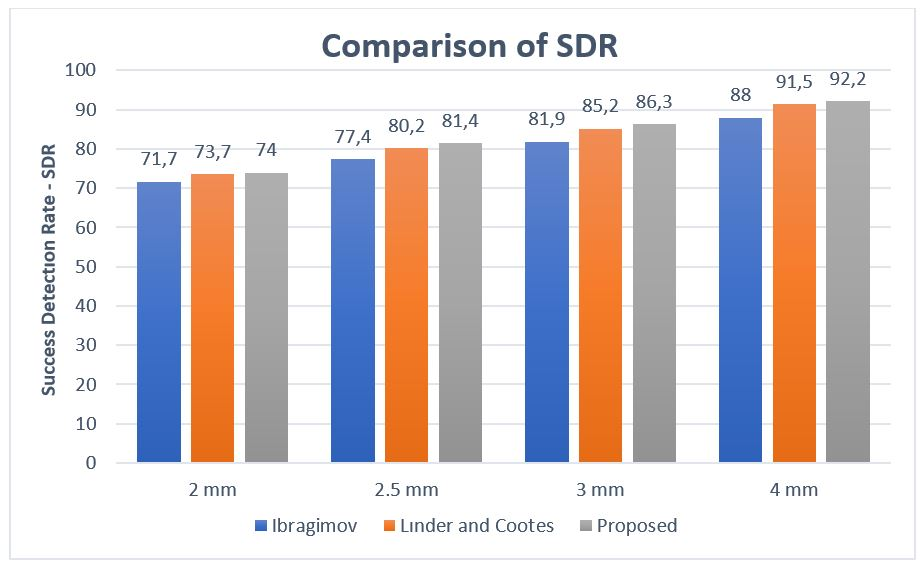
\includegraphics[width=5.76in]{./media/image4}
		\caption{Success Detection Rate (SDR) comparison of our model results with the results got by \cite{ref3} and \cite{ref8}}
		\label{fig4}
	\end{center}\vs{-4mm}
\end{figure}



%%%%%%%%%%%%%%%%%%%% Figure/Image No: 4 Ends here %%%%%%%%%%%%%%%%%%%%

\tab As shown in Figure (\ref{fig4}) above, the results of the model were compared with the results found by other experts based on the same dataset. \cite{ref4} was able to get a SDR of 71.7$\%$  on 2mm range, 77.4$\%$  on 2.5mm, 81.9$\%$  on 3mm and 88$\%$  on 4mm range. \cite{ref8} proposed method got 73.7$\%$  on 2mm range, 80.2$\%$  on 2.5mm, 85.2$\%$  on 3mm and 91.5$\%$  on 4mm range. \  Our proposed model, consisting of base model, achieved 74$\%$  SDR in the range of 2 mm. In the range of 2.5 mm, it resulted in a success detection rate of 81.4$\%$ , 86.3$\%$  in the 3 mm range and 92.2$\%$  in the 4mm range. It shows better results in all the evaluation metrics as shown in figure (\ref{fig4}) above. 

\section{Conclusions}
\tab A modified U-net model was proposed to address the problem of Cephalometric Analysis. Data Augmentation was applied on the training dataset and a total of 1350 images was trained to detect 19 anatomical landmark points coordinates. The SDR achieved through this framework shows success results as shown in figure (\ref{fig4}) above.  

\tab The proposed model performs better and give better results when compare to the results accepted during the competition launched by ISBI 2015. All models are trained using images with of size 256x256 to provide faster training and easier experiments. The uncertainty measurements used during this study, measurements based on the predictive variance, consistently work well and provide good results that can be used by physicians as evaluation metrics on specific tasks. This model can easily be implemented in a real computer aided cephalometric analysis applications that work with data from different devices. 


\section*{Acknowledgment}
The research was performed as a thesis topic to pursue Master degree in Computer Engineering from Konya Technical University, Faculty of Engineering and Natural Science, Konya/Turkey. \textbf{This work was fully supervised by Assoc. Prof. Betül Uzbaş.} 

\begin{thebibliography}{99}
	\bibitem{ref1} Qian, J., et al. CephaNet: An Improved Faster R-CNN for Cephalometric Landmark Detection. in 2019 IEEE 16th International Symposium on Biomedical Imaging (ISBI 2019). 2019. IEEE. 
	\bibitem{ref2} Yue, W., et al., Automated 2-D cephalometric analysis on X-ray images by a model-based approach. IEEE transactions on biomedical engineering, 2006. 53(8): p. 1615-1623.
	\bibitem{ref3} Lindner, C. and T.F. Cootes. Fully automatic cephalometric evaluation using random forest regression-voting. in IEEE International Symposium on Biomedical Imaging. 2015. Citeseer.
	\bibitem{ref4} Ibragimov, B., et al. Computerized cephalometry by game theory with shape-and appearance-based landmark refinement. in Proceedings of International Symposium on Biomedical imaging (ISBI). 2015.
	\bibitem{ref5} Cardillo, J. and M.A. Sid-Ahmed, An image processing system for locating craniofacial landmarks. IEEE transactions on medical imaging, 1994. 13(2): p. 275-289.
	\bibitem{ref6} Lee, H., M. Park, and J. Kim. Cephalometric landmark detection in dental x-ray images using convolutional neural networks. in Medical Imaging 2017: Computer-Aided Diagnosis. 2017. International Society for Optics and Photonics.
	\bibitem{ref7} Wang, C.-W., et al., A benchmark for comparison of dental radiography analysis algorithms. Medical image analysis, 2016. 31: p. 63-76.
	\bibitem{ref8} Lindner, C., et al., Fully automatic system for accurate localisation and analysis of cephalometric landmarks in lateral cephalograms. Scientific reports, 2016. 6: p. 33581.
	\bibitem{ref9} Jung, A.B., imgaug. Online; accessed 30-Oct-2018, 2018.
	\bibitem{ref10} Ronneberger, O., P. Fischer, and T. Brox. U-net: Convolutional networks for biomedical image segmentation. in International Conference on Medical image computing and computer-assisted intervention. 2015. Springer.
	\bibitem{ref11} Goutham, E., et al. AUTOMATIC LOCALIZATION OF LANDMARKS IN CEPHALOMETRIC IMAGES Via MODIFIED U-Net. in 2019 10th international conference on computing, Communication and Networking Technologies (ICCCNT). 2019. IEEE.
	\bibitem{ref12} Paszke, A., et al., Automatic differentiation in pytorch. 2017.
	\bibitem{ref13} Ye, Z., et al., Building Extraction from Very High Resolution Aerial Imagery Using Joint Attention Deep Neural Network. Remote Sensing, 2019. 11(24): p. 2970.
	\bibitem{ref14} Kingma, D.P. and J. Ba, Adam: A method for stochastic optimization. arXiv preprint arXiv:1412.6980, 2014.
	
\end{thebibliography}


\end{document}
